\documentclass{article}

% GRAPHICS
\usepackage{float}
\usepackage{subcaption}
\usepackage{tikz}
\usepackage{tikzscale}
\usetikzlibrary{calc}
\usepackage{graphicx}

% MATHS
\usepackage{amsmath}
\usepackage{gensymb}

\usepackage{mathtools}
\newcommand\coolover[2]{\mathrlap{\smash{\overbrace{\phantom{%
    \begin{matrix} #2 \end{matrix}}}^{\mbox{$#1$}}}}#2} 
\newcommand\coolunder[2]{\mathrlap{\smash{\underbrace{\phantom{%
    \begin{matrix} #2 \end{matrix}}}_{\mbox{$#1$}}}}#2}
    
\newcommand\coolleftbrace[2]{%
#1\left\{\vphantom{\begin{matrix} #2 \end{matrix}}\right.}

\newcommand\coolrightbrace[2]{%
\left.\vphantom{\begin{matrix} #1 \end{matrix}}\right\}#2}


% GRAPHICS
\usepackage{float}
\usepackage{subcaption}
\usepackage{tikz}
\usepackage{tikzscale}
\usetikzlibrary{calc}
\usepackage{graphicx}

% HYPERLINKS
\usepackage{hyperref}

% DOCUMENT PADDING AND MARGINS
\usepackage{titlesec}
\usepackage[margin=1.2in]{geometry}
\setlength{\parskip}{\baselineskip}%
\setlength{\parindent}{0pt}
\titlespacing*{\section}{0pt}{5ex}{2ex}
\titlespacing*{\subsection}{0pt}{1ex}{-2ex}
\titlespacing*{\subsubsection}{0pt}{2ex}{-2ex}

%COMMENTING
\usepackage{comment}


\begin{document}

% TITLE
\title{ME780 Assignment 2}
\author{Stan Brown \& Chris Choi}
\date{}
\maketitle

\section{Motion Model of a Bicycle}
Define the bicycle motion model for an Ackermann steered robot as shown in the configuration below(and presented in the motion modelling lecture notes). 
\begin{figure}[H]
	\centering
	\includegraphics[width=0.6\textwidth]{images/bicycle_model.png}
	\caption{Bicycle in World Frame}
	\label{fig:bicycle}
\end{figure}

From the lecture notes, the motion of front wheel can be written as follows:

\begin{align}
	x_{f} &= x + L \cos(\theta) \\
	y_{f} &= y + L \sin(\theta) \\
 	\begin{bmatrix}
        x_{f, t} \\
        y_{f, t} \\
    \end{bmatrix}  
    &=
    \begin{bmatrix}
	    x_{f, t - 1} + v_{f, t} \cos(\theta_{f, t - 1} + \delta_{t}) dt \\
		y_{f, t - 1} + v_{f, t} \sin(\theta_{f, t - 1} + \delta_{t}) dt \\
    \end{bmatrix}
\end{align}

Similarly the motion of the rear wheel is as follows: 

\begin{align}
 	\begin{bmatrix}
        x_{r, t} \\
        y_{r, t} \\
    \end{bmatrix}  
    &=
    \begin{bmatrix}
	    x_{r, t - 1} + v_{r, t} \cos(\theta_{r, t - 1}) dt \\
		y_{r, t - 1} + v_{r, t} \sin(\theta_{r, t - 1}) dt \\
    \end{bmatrix}
\end{align}

These two equations can be linked and simplified by using the Instantaneous Center of Rotation (ICR) to combine equations of motion for the front and rear wheels as follows.

\begin{figure}[H]
	\centering
	\includegraphics[width=0.6\textwidth]{images/bicycle_icr.png}
	\caption{Simplifying the Bicycle Model with ICR}
	\label{fig:bicycle_icr}
\end{figure}

From Fig~\ref{fig:bicycle_icr} the relationship between the steering angle $\delta$ relative to the bicycle's heading can be written as:

\begin{equation}
	\label{eq:icr_steering_angle}
	\tan(\delta) = \dfrac{L}{R}
\end{equation}

Moreover, we know that the angular velocity $\omega$ from the point ICR of both the front and rear wheel is:

\begin{equation}
	\label{eq:icr_angluar_velocity}
	\omega = \dfrac{v \tan(\delta)}{L} = \dfrac{v}{R}
\end{equation}

Now that we have the angular velocity of the bicycle over time, the bicycle's change in heading over time is simply:

\begin{equation}
	\theta_{t} = \theta_{t - 1} + \dfrac{v_{t} \tan(\delta_{t})}{L} dt
\end{equation}

For the complete motion model of the bicycle we have:

\begin{align}
 	\begin{bmatrix}
        x_{t} \\
        y_{t} \\
        \theta_{t}
    \end{bmatrix}  
    &=
    \begin{bmatrix}
	    x_{t - 1} + v_{t} \cos(\theta_{t - 1}) dt \\
		y_{t - 1} + v_{t} \sin(\theta_{t - 1}) dt \\
		\theta_{t - 1} + \dfrac{v_{t} \tan(\delta_{t})}{L} dt
    \end{bmatrix}
\end{align}

Using Equation 8, the bicycle motion model was simulated in Matlab over a period of 20 seconds with the following parameters:

\begin{itemize}	
	\vspace{-0.4cm}
	\setlength{\itemsep}{0pt}
	\setlength{\parskip}{0pt}
	\setlength{\parsep}{0pt}
	
	\item{Simulation time step $dt$: 0.1s}
	\item{Velocity $v$: $3 \text{ms}^{-1}$}
	\item{Length of bicycle $L$: 0.3m}
	\item{Steering angle $\delta$: $10 - t$ degrees}
	\item{Steering angle limit: $\pm 30$ degrees}
	\item{Standard deviation on $x$ and $y$: 0.02m}
	\item{Standard deviation on $\theta$: 1 degree}
\end{itemize}

The resulting trajectory from the simulation inputs is shown in Fig~\ref{fig:bicycle_20s}. Based on the simulation inputs the the observed trajectory appears to be valid as the heading starts at 10 degrees and then decreases at a rate of -1 degree per second. This means during the first half of the run the steering angle is positive, causing it to steer to the left, straighten out for a portion and then begin starting to turn to the right as the steering angle becomes negative. These motions result in the "S" shape that is depicted in  Fig~\ref{fig:bicycle_20s}




\begin{figure}[H]
	\centering
	\includegraphics[width=0.7\textwidth]{images/bicycle_motion_20s.jpg}
	\caption{Simulating the Bicycle Model for 20s starting from (0, 0)}
	\label{fig:bicycle_20s}
\end{figure}


\newpage
\section{Carrot Controller for Bicycle}

Develop a carrot following controller.  The way this controller works is you define a carrot, or point on the desired trajectory line a fixed distance, $r$, ahead of the closest point on the line to the current robot position.

\begin{figure}[H]
	\centering
	\includegraphics[width=0.6\textwidth]{images/carrot_controller.png}
	\caption{Carrot Controller}
	\label{fig:carrot_controller}
\end{figure}

A carrot controller is a controller that has a carrot point with a fixed distance $r$ on the trajectory line, ahead of the closest point on the trajectory line to the current robot position.


\subsection{Closest Point on the Trajectory Line to the Robot}
The closest point between the robot's position and the trajectory line can be calculated by first calculating the projection of the vector formed by the current location and the desired 

\begin{figure}[H]
	\centering
	\includegraphics[width=0.5\textwidth]{images/dot_product_projection.png}
	\caption{Dot Product Projection)}
	\label{fig:dot_product_projection}
\end{figure}

Let the vector $a$ denote the vector from the start of the trajectory line to the position of the robot, and vector $b$ denote the start and end of the trajectory line. To calculate the closest point on vector $b$ to the robot position one simply has to project vector $a$ onto vector $b$, this can be calculated via:

\begin{equation}
	\text{proj}_{\vec{a}\vec{b}} 
		= \dfrac{\vec{a} \cdot \vec{b}}{|\vec{a}|}
			\dfrac{\vec{a}}{|\vec{a}|} 
		= \dfrac{\vec{a} \cdot \vec{b}}{|\vec{a}|^{2}}
			\vec{a}
\end{equation}


\newpage
\subsection{Calculation of the Carrot Point}
Once the closest point on the trajectory line to the robot is found, calculating a carrot point along the trajectory line is the closest point on the trajectory line $p_{\text{closest}}$ plus the product of look ahead distance $r$ times the unit vector of the trajectory line $b$.

\begin{equation}
	\text{carrot} = p_{\text{closest}} + r \dfrac{\vec{b}}{|\vec{b}|}
\end{equation}



\subsection{Carrot Controller}
We implemented a proportional (P) carrot controller and traced a rectangle of $20m$ by $5m$ at $3ms^{-1}$. This is the resulting motion of the bicycle (See Fig~\ref{fig:bicycle_carrot}), we used a proportional gain $k_{p} = 2$ and look ahead distance $r$ at $2$, $0.2$ and $5$. 

From Fig~\ref{fig:bicycle_carrot} we can see that different look ahead distance $r$ impacts the way the robot traces a rectangle. If the look ahead distance is too low (i.e. Fig~\ref{fig:bicycle_carrot_bad} where $r = 0.2$), the carrot will be a very small distance ahead of the robot, making small adjustments unlikely thereby the angle of the steering oscillates between $-30$ degrees to $30$ degrees (the max steering angle).

If the carrot is at a medium look ahead distance away from the robot  (i.e. Fig~\ref{fig:bicycle_carrot_ok} where $r = 2$), the robot tends to be quite agreessive in compensating for overshooting the trajectory. As we increase the look ahead distance $r$ however, the correction angle is dampened, causing a less agreessive correction, but longer time to return to the trajectory line.

\begin{figure}[H]
	\centering
	
	\begin{subfigure}[b]{\linewidth}
		\centering
		\includegraphics[width=0.5\textwidth]{images/bicycle_carrot_bad.jpg}
		\caption{$k_{p} = 2$, $r = 0.2$}
		\label{fig:bicycle_carrot_bad}
	\end{subfigure}
		
	\begin{subfigure}[b]{\linewidth}
		\centering
		\includegraphics[width=0.5\textwidth]{images/bicycle_carrot.jpg}
		\caption{$k_{p} = 2$ and $r = 2$}
		\label{fig:bicycle_carrot_ok}
	\end{subfigure}
	
	\begin{subfigure}[b]{\linewidth}
		\centering
		\includegraphics[width=0.5\textwidth]{images/bicycle_carrot_better.jpg}
		\caption{$k_{p} = 2$, $r = 5$}
		\label{fig:bicycle_carrot_better}
	\end{subfigure}
	
	\caption{Bicycle motion using carrot controller starting at (23, 10)}
	\label{fig:bicycle_carrot}
\end{figure}



\newpage
\section{IGVC Planner}
\label{sec:igvc_planner}
We were given a map of the Intelligent Ground Vehicle Competition in the form of a $926 \times 716$ element grid, where each cell
represents a 10 cm X 10 cm area of the course, resulting in a 92.6 m X 71.6 m environment. 

Our goal is to implement a planner and present a combined motion planning solution that finds a straight-line path through the environment, then uses the carrot controller to provide the inputs required to drive the robot to the start and end locations which are ocated at ($x = 4.0m$, $y = 0.5m$, $\theta = 3.14159 rad$) and ($x = 5.0 m$, $y = 1.0 m$, $theta =$ not defined) respectively. 


\begin{figure}[H]
	\centering
	\includegraphics[width=0.7\textwidth]{images/IGVCmap.jpg}
	\caption{IGVC Map}
	\label{fig:igvc_map}
\end{figure}



\newpage
\subsection{Wavefront Planner}
\label{subsec:wavefront}
Since the map given represents an occupancy grid of free space and obstacles, our initial approach to the planning portion was to apply the wavefront a path that finds an optional path between start to goal point. Fig~\ref{fig:wavefront} highlights the results of the wavefront planner and highlights the resulting path found by gradient decent. 
\begin{figure}[H]
	\centering
	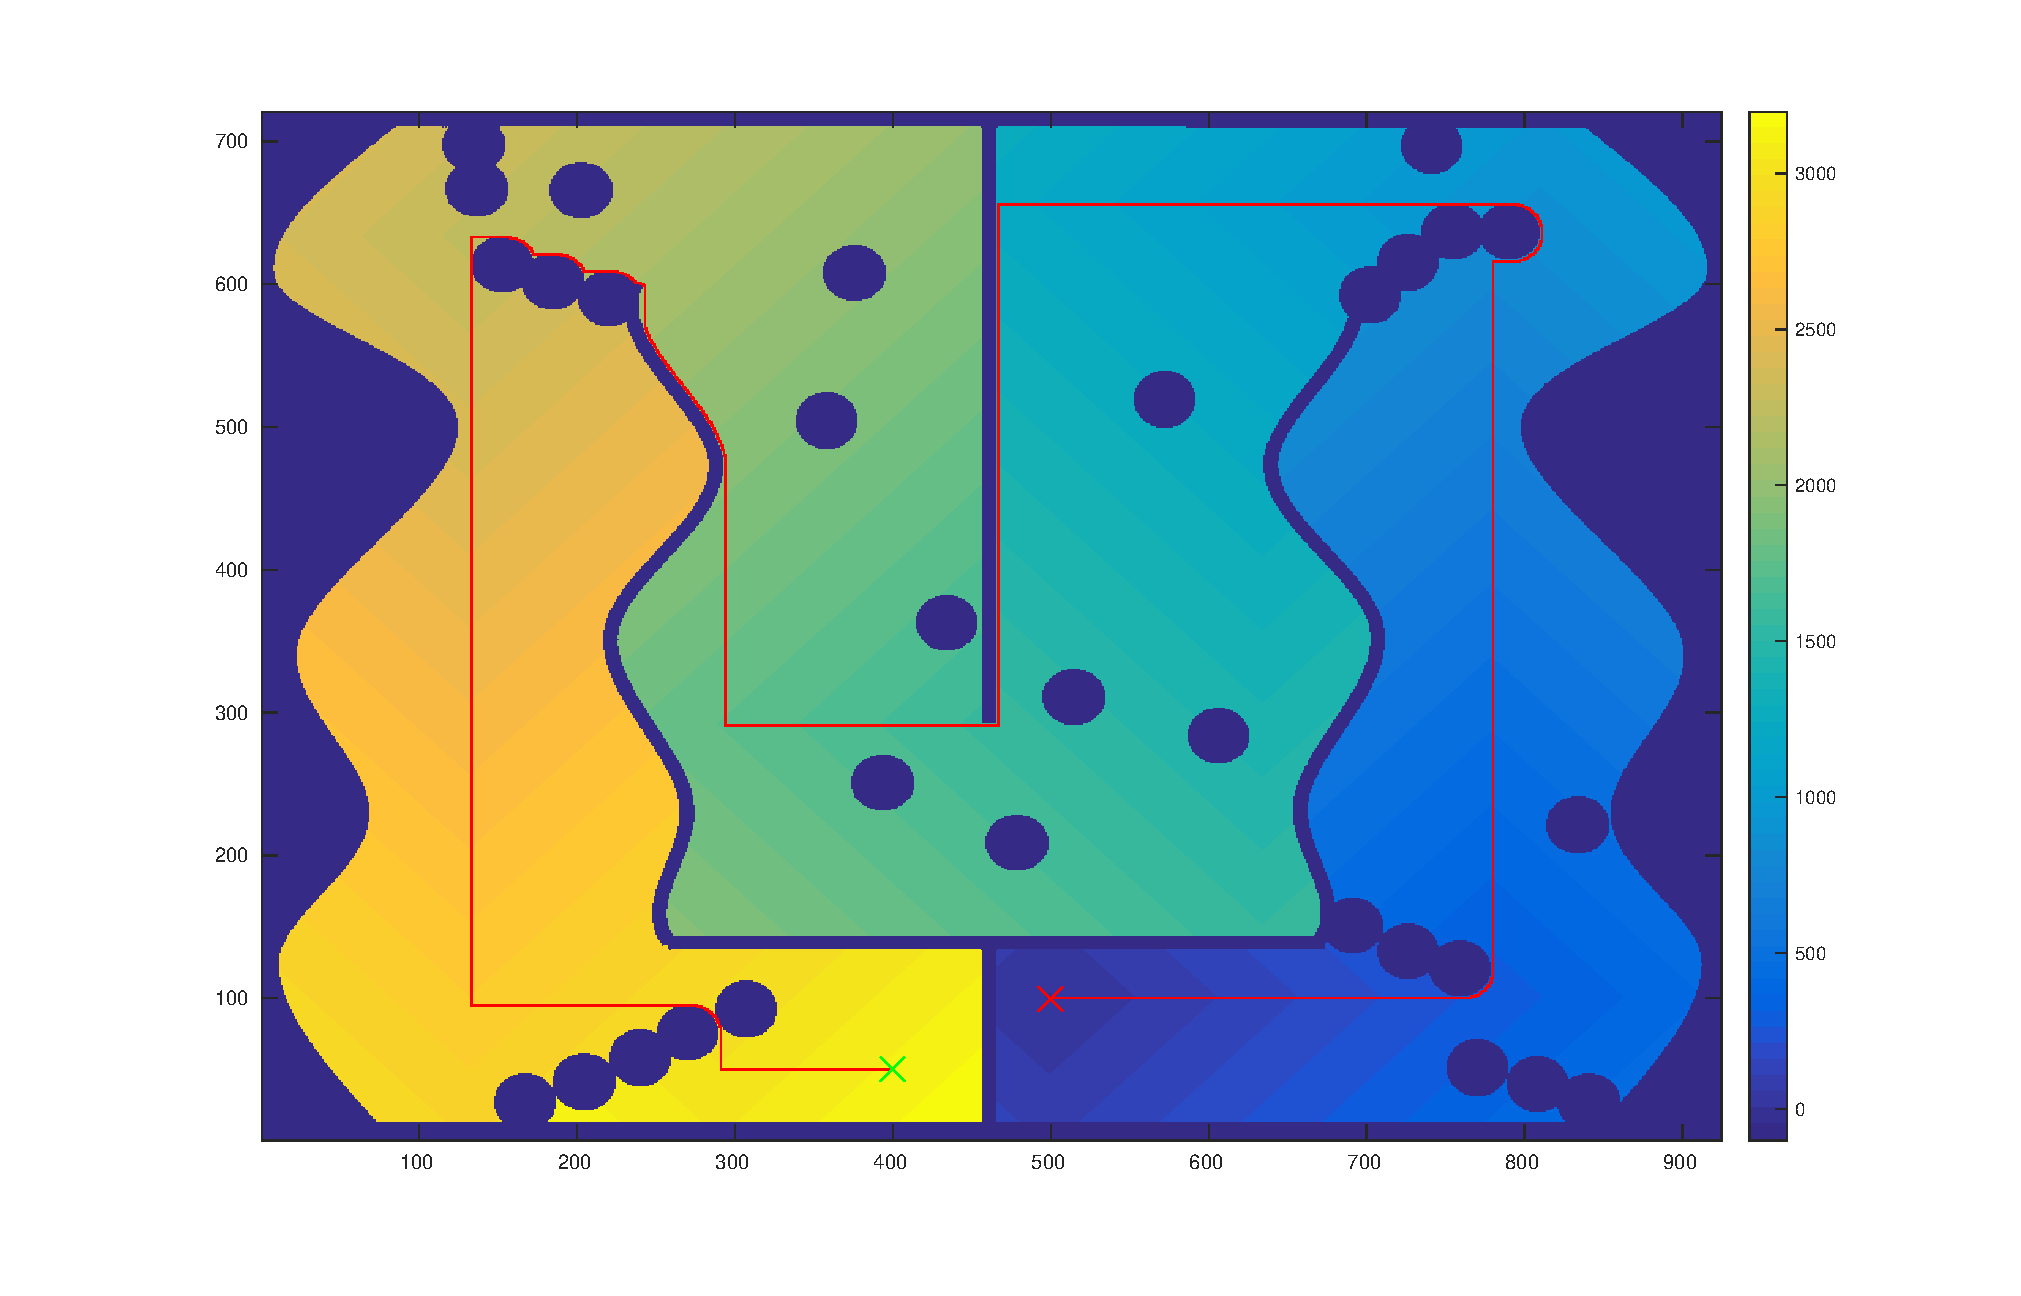
\includegraphics[width=0.9\textwidth]{images/wavefront_igvc.eps}
	\caption{Wavefront IGVC Map}
	\label{fig:wavefront}
\end{figure}

While the wavefront method successfully found an optimal solution on the grid based environment, it is far from optimal then a path generated in the continuous space. This problem stems from the fact that wavefront method is a grid based method based on a breadth first search that starts and the end goal and calculates a distance between the end goal and all points in the map. Because the distance is based on the number of grids between the start and end point the distance calculated actually reflects the Manhattan Distance between the start and end goals rather than the Euclidean Distance. This means that driving at a $45^o $ angle has the same distance as two paths that first travel horizontal and then upward. Furthermore the robots trajectory is restricted to the exploration directions used to generate the wavefront which in this case were a set 4 moves, mainly move up, move right, move left and move down. 

Additional problems are realized when one takes into account that the fact that robot is likely larger than the grid cells which makes collision avoidance and detection difficult. In many cases the grid cells are assumed to be the size of the robot but this has the additional drawback of causing obstacles to become very course and poorly represented. In Fig~\ref{fig:wavefront} it can be noted that the wavefront planner slips between a very small gap between two pylons on the course, which unless the robot is 10cm by 10cm, would be an impossible path for the robot to follow. Additionally the robot also tends to hug obstacles very closely which means that any errors in possession or heading are likely to result in collisions. 

Lastly, for this large map, the run time was over 40 seconds without any collision checking procedures and therefore this approach was abandoned in favour of a Probabilistic Roadmap Planner (PRM). 


\subsection{Probabilistic Roadmap Planner}
\label{subsec:prm}
In our next approach we used the Probabilistic Roadmap (PRM) planner, purely out of curiosity and it seemed like an intuitive alternative to wavefront planner. 

For the PRM implementation on a grid based environment, we had to make modifications to the provided PRM example, which assumes the obstacles are in the form of set of polygon points. This allows the PRM planner implemented in the ME 597 example code to exploit Matlab's \textit{inpolygon }function to detect whether a sample point located within a polygon. 

However the map given in this assignment is represented an occupancy grid instead of set of polygons, and therefore the collision checking portion of the PRM code to be replaced by a ray tracing algorithm. In our implementation we utilized a modified version of Bresenham's line algorithm, to find create collision free edges between sample points.

We implemented a PRM planner and then applied the carrot controller outlined in Question 2 to the resulting paths which are shown in  Fig~\ref{fig:prm} which also highlights the effect of using varying sample sizes in the PRM. From testing it appears that a sample size of 200 will yield a valid solution in about 50 percent of the time, a sample size of 500 will yield a solution is 90 percent of cases and a sample sizes with more than 1000 sample points always resulted in a solution. 

Higher sample sizes also tended to lead to smoother and more optimal paths which can be observed by comparing  the 200 sample case to the 5000 sample case highlighted in Fig~\ref{fig:collision_example}. The run time of the PRM when using 5000 points less than 3 seconds which is a significant improvement over the wavefront planner which took over a minute to find a solution.  


\begin{figure}[H]
	\centering
	\begin{subfigure}[b]{0.49\linewidth}
		\centering
		\includegraphics[width=\textwidth]{images/prm_200.jpg}
		\caption{200 Samples}
	\end{subfigure}
	\begin{subfigure}[b]{0.49\linewidth}
		\centering
		\includegraphics[width=\textwidth]{images/prm_500.jpg}
		\caption{500 Samples}
	\end{subfigure}
	
	\begin{subfigure}[b]{0.49\linewidth}
		\centering
		\includegraphics[width=\textwidth]{images/prm_1000.jpg}
		\caption{1000 Samples}
	\end{subfigure}
	\begin{subfigure}[b]{0.49\linewidth}
		\centering
		\includegraphics[width=\textwidth]{images/prm_5000.jpg}
		\caption{5000 Samples}
	\end{subfigure}
	\caption{PRM Planner and Carrot Controller}
	\label{fig:prm}
\end{figure}



\subsubsection{PRM Planner with Sample Points Padded}
\label{subsec:prm_padding}

While the PRM yielded a complete path between teh start and end goals, it was noted that at some locations along the path the robot will pass extremely close to obstacles due to the PRM cutting the corners extremely tightly. This behaviour is due to a lack of particles in locations near choke points. An example of the PRM cutting a corner to tightly is highlighted in  Fig~\ref{fig:prm}. 

\begin{figure}[H]
	\centering
	\includegraphics[width=\linewidth]{images/collision_example.jpg}
	\caption{Collision Example}
	\label{fig:collision_example}
\end{figure}


We attempted to address this issue by adjusting the way that sample points were created in the PRM planner by checking for any obstacles within that are within 0.5 m circle  of each sample point. If an obstacle is detected with 0.5 m of a point, the point is deleted and a set of 5 additional points are created and randomly distributed within a circle centred at the deleted sample point with a radius of 1.5 m. These points are again checked for proximity to obstacles and pruned in a the same manner described as above. 

This approach resulted in areas near walls and obstacles to be sampled much more heavily compared to open spaces and also resulted in smoother paths near obstacles and are highlighted in Fig~\ref{fig:prm_resampling}


\begin{figure}[H]
	\centering
	\includegraphics[width=\linewidth]{images/prm_resampling.jpg}
	\caption{PRM Resampling with 1000 points and a collision check raduis of 0.5 m}
	\label{fig:prm_resampling}
\end{figure}


\section{Limitations and Future Improvements to the PRM Planner}
\subsection{Limitations}

Previously in Section~\ref{sec:igvc_planner}  explored both wavefront and PRM path planning methods, both methods alone are not satisfactory in planning a path for the bicycle through the IGVC course, we will discuss three limitations below along with possible solutions:

\begin{itemize}

	\item{\textbf{Path is not smooth}: The paths generated by both wavefront and PRM do not account motion model of the bicycle. Some portions of the planned paths have very sharp edges or corners, particularly in locations near very sharp obstacles such as the wall located in the middle of the course. Such an angle is to sharp for the controller and therefore results in a non optimal turn around the obstacle that could be avoided if the planner could take into account the robots turning radius. 	
}
	
\item{\textbf{No collision detection}: None of the explored methods explicitly perform collision detection of a robot with an actual size. We approximated some collision checking using our re-sampling approach which did eliminate a significant portion of collisions but not all of them. One possible way to perform collision checking in the PRM approach would be to modify the A* search algorithm to check for collisions with obstacles when selecting an edge to transverse. One option for collision checking would be to check parallel line segments located at a distance 0.5 robot widths above and below the line segment formed by a selected edge for collision. If one of these lines was to found to interest an obstacle the edge should not be added to the final path.  
}

\item{\textbf{Map is assumed to be known, accurate and static}: Probably the largest limitation to our approach is the assumption that the map is accurate and static. A local planner such as trajectory roll-out combined with some kind of range sensor, such as lidar, would allow the robot to determine paths that avoid uncounted for obstacles. In the case of non-static obstacles, such as other robots (since it is a race) a real time object tracker could be implemented and used to make predictions as to where moving obstacles will be in future which could then be used by the local planner to come up with a collision free trajectory. 
}
	
\end{itemize}





\end{document}